\documentclass[12pt]{article}
\usepackage[utf8]{inputenc}
\usepackage[margin=1in]{geometry}
\usepackage{setspace}
    \doublespacing
\usepackage{lipsum}
\usepackage{enumitem}
\usepackage{booktabs}
\usepackage[style = apa]{biblatex}
    \addbibresource{RE.bib}
\usepackage{titlesec}
    \titleformat{\section}{\normalsize\bfseries}{}{0pt}{}
    \titlespacing*{\section}
        {0pt}{12pt plus 4pt minus 2pt}{0pt plus 2pt minus 2pt}
\usepackage{pgfplots}
    \usepgfplotslibrary{dateplot}
    \pgfplotsset{ every non boxed x axis/.append style={x axis line style=-} }
    \pgfplotsset{compat=1.15}
    \pgfplotsset{compat = newest}
    \usetikzlibrary{positioning, arrows.meta}
    \usepgfplotslibrary{fillbetween}
\usepackage{tikz}
\usepackage{float}
\usepackage{fancyhdr}
\usepackage{hyperref}
\usepackage{mathptmx}
\usepackage{multirow}
\usepackage{ulem}
\usepackage{amsmath}
\usepackage[labelsep=period]{caption}
\usepackage{graphicx}
    \graphicspath{{./Graphs/eps}}
\usepackage[figurename=Figure]{caption}
        \DeclareCaptionFormat{figure}
            {
                \small #1#2#3
            }
    \captionsetup{format=figure}

\begin{document}

\begin{center}
{\LARGE \textbf{Regional resilience in Italy during COVID-19 and measures of resilience}}
        
\vspace{0.4cm}
{\large Mario Patanè}

\vspace{0.4cm}

{\large January 2023}
\end{center}
\vspace{0.4cm}
\begin{onehalfspace}
\begin{abstract}
    \vspace{0.2cm}
    \centering
    \begin{minipage}{5in}
        This work aims to measure the resistance and recoverability aspects of resilience in Italy NUTS-2 regions in the context of the exogenous shock originated from COVID-19 using simple statistical indices and to evaluate the current feasibility of an evaluation process in policy-making based upon a composite index that aggregates regional variables in an accurate measure of resilience, permitting regionally-tailored and heterogeneous policies.
    \end{minipage}
\end{abstract}
\end{onehalfspace}
\vspace{0.2cm}





\section{Introduction}

Recessions can be considered as unexpected and unpredictable events that disrupt the growth path of an economy. A recent example of recession was the one caused by the COVID-19 pandemic, a global health crisis that started in December 2019, and that was followed by government measures adopted in order to slow the spread of the contagion which turned it into a global economic crisis, sparked by the contraction of demand and disruption of supply and fueled by constant uncertainty (\cite{meinen_regional_2021}).

The subsequent macroeconomic downturn has been characterized by a major intra- and inter-country heterogeneity due to the diverse incidence of the disease and the related governments’ containment measures.
In this scenario of a spatially uneven impact, the notion of resilience seems fitting. Although resilience doesn't have a universally agreed definition, it can broadly be defined as how a system responds to external disturbances. Martin (\citeyear{martin_regional_2012}) initially analysed three main dimensions of resilience: resistance (sensitivity to shocks), recoverability (the extent and nature of recovery from the shock) and reorientation/renewal (the ability to adapt in response to a shock and to return to the long-run growth path).
This work explores those aspects of resilience through a descriptive analysis of the COVID-19 shock in order to measure its impact on Italy NUTS-1 (macro-regions) and NUTS-2 (regions), using simple indexes and attesting the diversity in responses across regions. 

Finally, we will evaluate the use of compound indices for measuring regional resilience and the potential implications in policy-making, in particular by verifying the general consensus in literature on the usage of regional resilience frameworks in policy-making, which could hypothetically enable regionally-tailored and heterogenous policies weighted on the regional inherent characteristic and growth paths and consequently on the amount of resilience estimated by said ideal index.

\section{Observing the consequences of COVID-19 in Italian regions with time series}

To get an overview of the effects of the COVID-19 exogenous shock, I used data from the Italian national institute of statistics (ISTAT) on the national seasonally adjusted GDP between 2016 and 2022. The temporal proximity of the event to the time of this writing suggests the use of a tighter time frame that would allow a more recent performance observation. Notwithstanding this choice appears the most fitting to our scenario, the unavailability of tight regional data led me to use an annual time frame instead for the following regional analysis. Another choice to be faced was taking into consideration either employment or income movements. Although previous influential works on resilience took into consideration employment as an insightful indicator of the outcome of complex adjustments in the local labour market and therefore of resilience (\cite{martin_regional_2012}; \cite{fingleton_recessionary_2012}), the case of Italy's labour market, which exhibit an homogeneity across regions due to institutional rigidities, makes GDP a more appropriate measure of resilience behaviours (\cite{cellini_regional_2014}, p. 4).

Figure \ref{fig:GDPita} shows the impact of the shock originated from the pandemic nationally; the clear contraction starts to appear on the first quarter of 2020 and has its trough at the beginning of the second quarter. Effects on NUTS-1 regions are shown in Figure \ref{fig:GDPN1}, which displays a significantly homogenous response to the shock, with the Central region enduring the most substantial impact. This is a surprising result; although the history of recessionary shocks in Italy seems to resolve in very few cases of heterogenous reactions (\cite{cellini_regional_2014}, p. 16), in this scenario, both the diverse regional spread of infections but even more so the specific regions’ sectoral structure (determining the impact of containment measures on sectors which do not allow to engage in social distancing or remote working) should be rather drivers of heterogeneity across regions (\cite{meinen_regional_2021}, p. 16; \cite{ascani_geography_2021}, p. 32). Taking into account a more local perspective through NUTS-2 territories in Figure \ref{fig:GDPN2}, the same uniform response appears.

\begin{figure}
    \centering
    \begin{minipage}[t]{.5\textwidth}
    \centering
    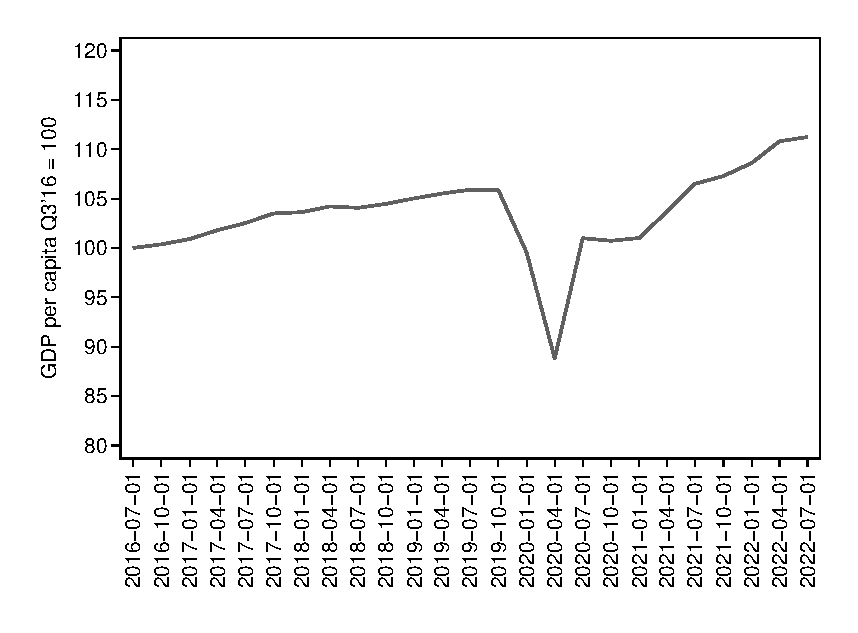
\includegraphics[width=\textwidth]{ita_gdpq.eps}
    \caption{Quarterly GDP per capita in Italy before and after COVID-19, (Q3'16 - Q3'22). \textit{Source}: Author's elaboration of ISTAT (\citeyear{istat}).}
    \label{fig:GDPita}
    \end{minipage}\hfill
    \begin{minipage}[t]{.5\textwidth}
    \centering
    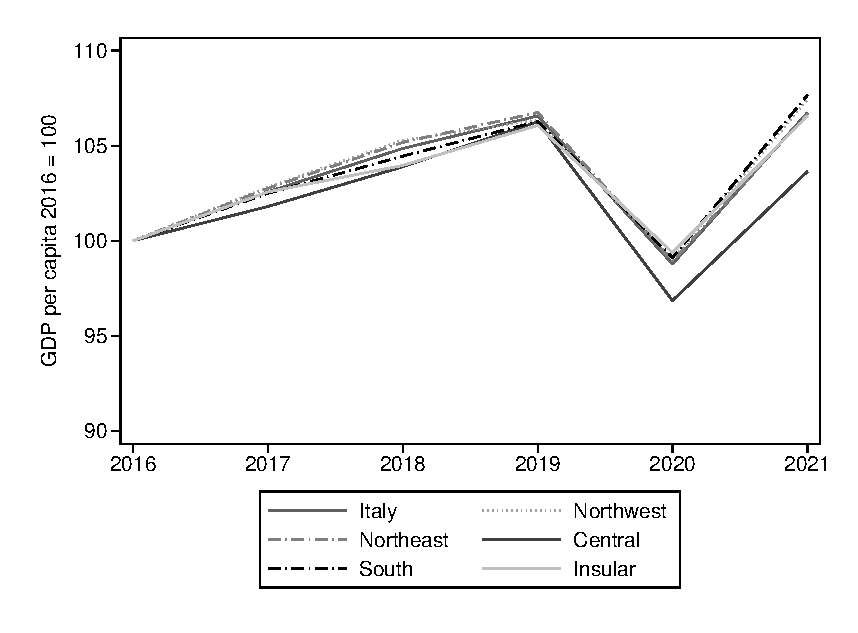
\includegraphics[width=\textwidth]{n1_gdpy}
    \caption{Annual GDP per capita in Italy's NUTS-1 regions before and throughout COVID-19, (2016-2021). \textit{Source}: Authors’ elaboration of ISTAT (\citeyear{istat}).}
    \label{fig:GDPN1}
    \end{minipage}
\end{figure}

\begin{figure}[H]
        \centering
        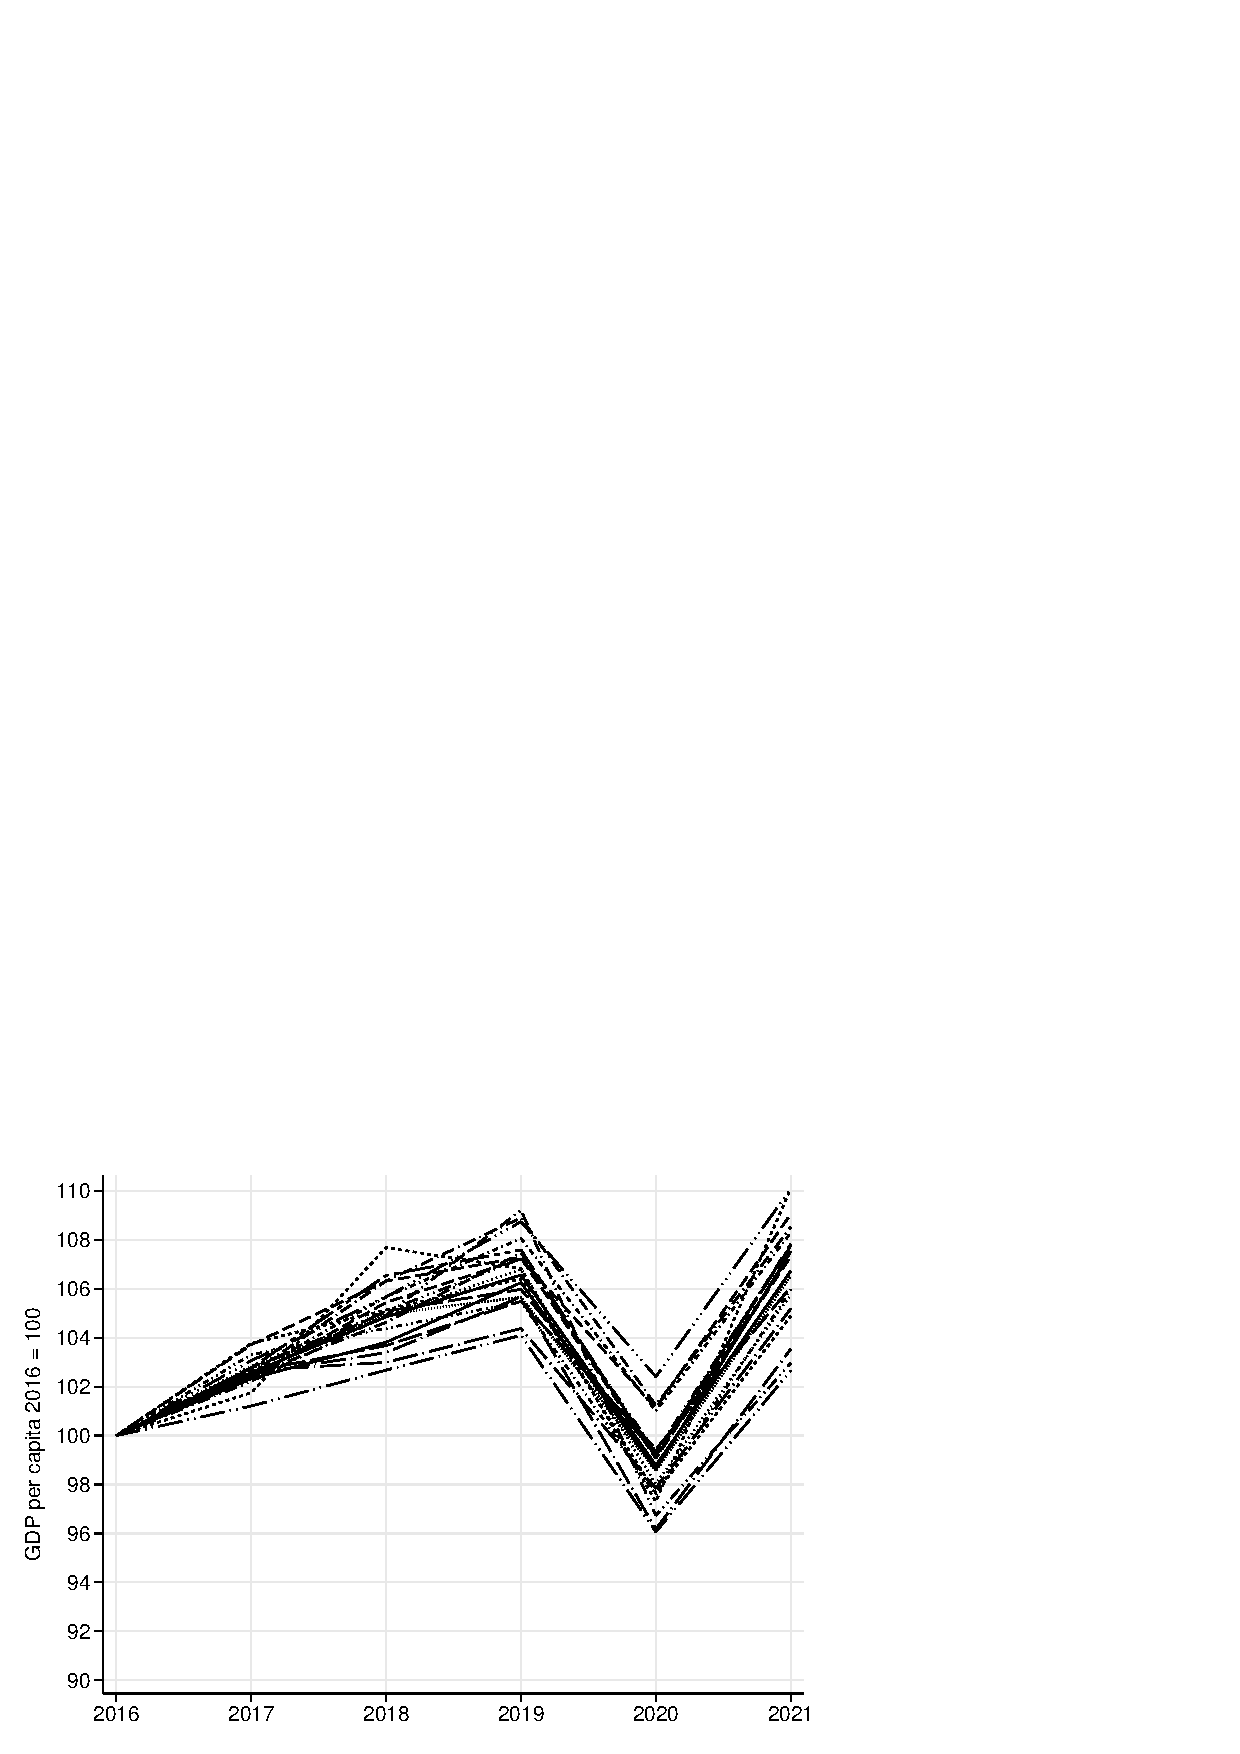
\includegraphics[width=250pt]{n2_gdpy.pdf}
        \caption{Annual GDP per capita for Italy's NUTS-2 regions before and throughout COVID-19, (2016-2021). \textit{Source}: Authors’ elaboration of ISTAT (\citeyear{istat}).}
        \label{fig:GDPN2}
\end{figure}
    


\section{Measuring resilience following COVID-19 across Italy's regions}
The observations that emerged in the previous section leads us to expect an homogeneous capacity of resistance and recovery across regions. To measure the resistance aspect of resilience in the regions I utilized a simple but effective measure proposed by Martin (\citeyear{martin_regional_2012}):

\begin{equation}
    \beta = \frac{\Delta GDP_{r}}{GDP_{r}}/\frac{\Delta GDP_{N}}{GDP_{N}}
\end{equation}

That is, the ratio of the relative difference in output for a region with respect to the relative difference in output for the country. The measure is centred around one, and when considering the relative difference between before and during the contraction, a value higher than one indicates a low resistance to the recessionary shock relative to the country, while a value of the index lower than one may indicate an higher resistance.

When measuring the recovery aspect, we are considering the difference between the peak in output following the contraction to its trough. We shall indicate this measure with \textit{$\gamma$}: a value higher than one may indicate a greater rebound of the region relative to the country, while values lower than one may indicate a sluggish recovery from the shock (relative to the country).

I calculated both the \textit{$\beta$} and \textit{$\gamma$} measures for NUTS-1 and NUTS-2 regions. Table \ref{tab:resnuts1} gives an overview per macro-regions that seems to average out the responses. The Central region appears the worst-performing with the highest sensitivity to the initial shock, and a muted recovery phase. As for the other macro-regions, they have been impacted quite similarly, with the Northern regions showing a mild rebound.


\begin{table}[h]
    \begin{center}
    \begin{tabular}{@{}llll@{}}
    \toprule[0.5pt]
    NUTS      &      & Sensitivity (\textit{$\beta$}) & Recovery (\textit{$\gamma$}) \\ \midrule[0.5pt]
    ITC      & Northwest & 0.92       & 1.08     \\
    ITH      & Northeast & 0.97       & 1.02     \\
    ITI      & Central   & 1.21       & 0.90     \\
    ITF      & South     & 0.96       & 1.00     \\
    ITG      & Insular   & 0.92       & 0.85     \\ \bottomrule[0.5pt]
    \end{tabular}
    \end{center}
    \caption{Sensitivity and recovery indexes for Italy NUTS-1 regions throughout COVID-19, (2020-2021). \textit{Source}: Author's elaboration of ISTAT \citeyear{istat}}
    \label{tab:resnuts1}
\end{table}

A more varied (while unsurprisingly similar) outcome is shown in Table \ref{tab:resnuts2}, in which the geographical disaggregation shows several uneven impacts within the same macro-region, for example in the South, where Basilicata and Sicily have a divergence in the coefficient of almost 0.5. The most sensitive region appears to be Tuscany, with also one of the lowest recovery measure, confirming the tough toll of COVID-19 on Central regions.

\begin{table}[h]
    \begin{center}
        \begin{tabular}{@{}llll@{}}
        \toprule[0.5pt]
        NUTS      &     Region                          & Sensitivity (\textit{$\beta$})  & Recovery (\textit{$\gamma$})    \\ \midrule[0.5pt]
        ITC1      & Piemonte                      & 1.06 & 1.01 \\
        ITC2      & Valle d'Aosta                 & 1.15 & 0.90 \\
        ITC3      & Liguria                       & 1.25 & 0.99 \\
        ITC4      & Lombardia                     & 0.82 & 1.11  \\
        ITF1      & Abruzzo                       & 1.05 & 1.02 \\
        ITF2      & Molise                        & 0.90 & 0.72 \\
        ITF3      & Campania                      & 1.01 & 1.01 \\
        ITF4      & Puglia                        & 0.82 & 1.00 \\
        ITF5      & Basilicata                    & 1.30 & 1.60 \\
        ITF6      & Calabria                      & 0.94   & 0.76 \\
        ITG1      & Sicilia                       & 0.84 & 0.79 \\
        ITG2      & Sardegna                      & 1.11 & 1.00 \\
        ITH1/2 & Trentino Alto Adige/S{\"u}dtirol & 0.88 & 0.97 \\
        ITH3      & Veneto                        & 1.10 & 1.05 \\
        ITH4      & Friuli-Venezia Giulia         & 0.90 & 0.93 \\
        ITH5      & Emilia-Romagna                & 0.88 & 1.02 \\
        ITI1      & Toscana                       & 1.54 & 0.88 \\
        ITI2      & Umbria                        & 1.09 & 1.06 \\
        ITI3      & Marche                        & 1.03 & 1.02 \\
        ITI4      & Lazio                         & 1.06 & 0.87 \\ \bottomrule[0.5pt]
        \end{tabular}
    \end{center}
    \caption{Sensitivity and recovery indexes for Italy NUTS-2 regions throughout COVID-19, (2020-2021). \textit{Source}: Author's elaboration of ISTAT \citeyear{istat}}
    \label{tab:resnuts2}
\end{table}

Updated indicators and medium-to-long-term series appear essential to precisely attest any hysteretic effect both at regional and national level; indeed several other factors could affect and have affected the growth path of economies since the pandemic, such as 2021 supply shocks and subsequent inflationary episodes which persists at the time of this writing (\cite{ubide2022inflation}).

Figures \ref{fig:scatn1} and \ref{fig:scatn2} plot the relationship between the sensitivity and recovery measures for each region, dividing the relationship into quadrants around the national values.

\begin{figure}{H}
    \centering
    \begin{minipage}[t]{.45\textwidth}
    \centering
    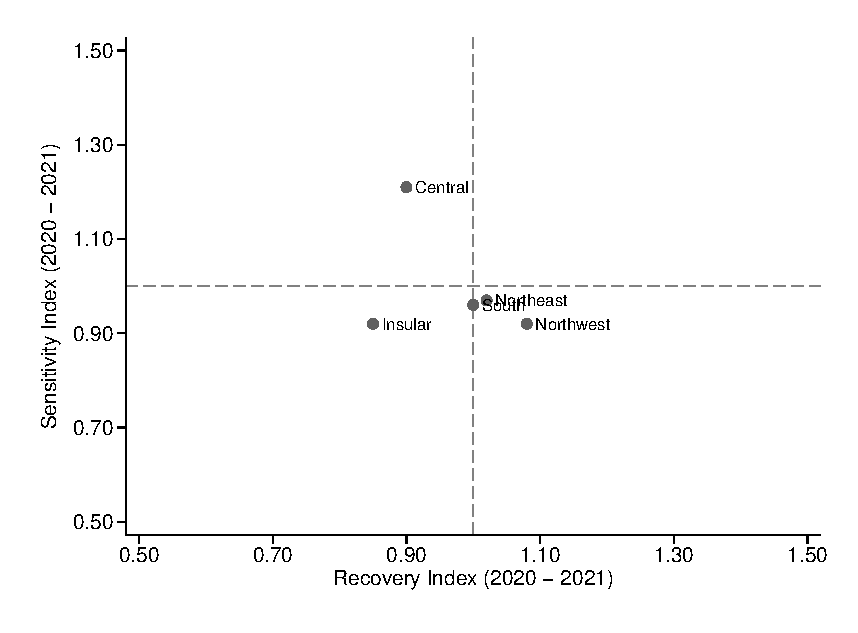
\includegraphics[width=\textwidth]{scatb.eps}
    \caption{Sensitivity and recovery indexes for Italy's NUTS-1 regions throughout COVID-19. \textit{Source}: Author's elaboration of ISTAT (\citeyear{istat}).}
    \label{fig:scatn1}
    \end{minipage}\hfill
    \begin{minipage}[t]{.45\textwidth}
    \centering
    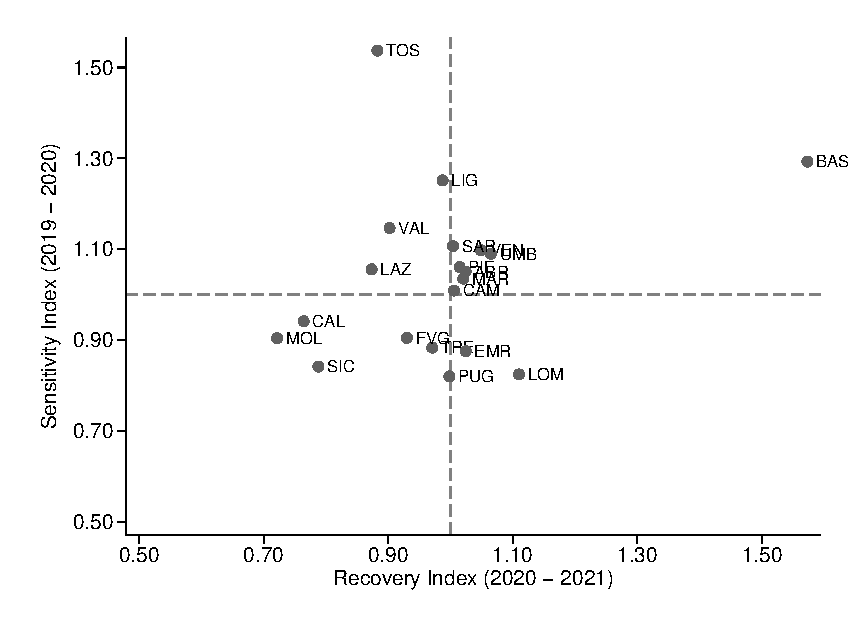
\includegraphics[width=\textwidth]{scatn2.eps}
    \caption{Sensitivity and recovery indexes for Italy's NUTS-2 regions throughout COVID-19. \textit{Source}: Authors’ elaboration of ISTAT (\citeyear{istat}).}
    \label{fig:scatn2}
    \end{minipage}
\end{figure}

Examining the NUTS-2 representation, it appears that no clear relationship is present, as less resistant regions performed dissimilarly on the recovery side. The case of Tuscany and Basilicata is the most evident, with the first one performing as we would expect, affected by an heavy impact and with a slower recovery, whereas Basilicata after the weak resistance to the impact, quickly 'bounced back'. South and Insular regions show a lower sensitivity to the shock despite struggling to grow afterwards. The first and second most productive regions of Italy, Lombardy and Lazio, showed opposite behaviours, as Lombardy performed more resistantly and recovered faster, while Lazio was slightly more impacted compared to the national level while also recovering slower. These observations are seemingly coherent with works analyzing the exposure related to the peculiarity of value chains. Ferraresi et al. (\citeyear{ferraresi_economic_nodate}) found that:
\begin{quote}
(\dots) Southern regions, whose degree of specialization in essential consumption value chains is higher than northern ones, may have suffered relatively less losses from the lockdown closures during the first wave of contagion in Spring 2020. Moreover, northern regions, whose production systems are more embedded in investment- and export-related supply chains, have been highly exposed to mandatory social distancing measures and the related costs. At the same time, remote working potential, relatively higher in northern regions, may have acted as a mitigating factor.
\end{quote}
This might explain a degree of diversity across regions, although the differences founds in regional resilience appear not vast enough to call for a significant heterogeneous resilience to the COVID-19 shock, consistently with our initial hypothesis.

\section{Can resilience become a tool in the hand of political economy?}

The indexes elaborated in the previous analytical section, although in a simple but functional form, may spur the idea for more complex indexes having concrete use in the normative field. The question that comes into mind is then: should regional resilience be contained in the realm of retrospective analysis or are the times mature for it to become an effective tool for regionally tailored policies, helping regions with different growth paths and characteristics, recover from exogenous shocks? Can resilience indexes, serve in the process of shaping policies and help mitigating the impact of recessionary events?


First of all, the lack of an universal consensus towards a resilience index is not helpful. We can consider resilience as a multi-dimensional concept made up of different factors, and so it would be wise to measure it using a composite index, an already controversial topic by itself. A definition of composite index by the OECD (\citeyear{oecd_handbook_2008}) is: \textit{'when individual indicators are compiled into a single index on the basis of an underlying model'}. Composite indices (CI) have divided the literature between so-called 'aggregators' who see a value in combining indicators, and 'non-aggregators' who warn against the subjective nature of the weighting process and potential misinterpretation of indices (\cite{sharpe_literature_2004}). Despite this fracture, 'the advantages of CIs are clear, and they can be summarized in the unidimensional measurement of the phenomenon, an easy interpretation with respect to a battery of many individual indicators and simplification of the data analysis' (\cite{stanickova_understanding_2018}, p. 238). This last argumentation compels us to choose a composite index as measure of resilience, acknowledging that subjectivity in the weighting process may be a first critical issue of our hypothetical index.

Briguglio et al. (\citeyear{briguglio_economic_2009}) attempts to construct a composite index for resilience and notes that the criteria for the variables that compose the index were based upon 'appropriate coverage, simplicity and ease of comprehension, affordability, suitability for international comparisons and transparency'. To capture the effects of shock absorption or shock-counteraction policies across countries, proposes the four components of a resilience index: macroeconomic stability, microeconomic market efficiency, good governance and social development, and computes them by taking an simple average of the four components.
Pontarollo and Serpieri (\citeyear{pontarollo_composite_2020}) takes a similar approach, developing a composite synthetic index called Regional Resilience Indicator that defines the resilience lifecycle and monitors the regional degree of resilience capacity.
Stanickova and Meleck{\'y} (\citeyear{stanickova_understanding_2018})  after reviewing advantages and disadvantages of regional CIs, proposes a composite weighted index of regional resilience (CWIRR), approaching objectivity through an entropy method of criteria weighting. The authors conclude:
\begin{quote}
    The construction of a regional resilience index could have important policy implications and be used to support the decision-making of regional policy-makers, especially for setting directions and justifying the choice of priorities for building the resilience of regions in future.
\end{quote}

But could those hypothetical policy implications be universally agreed? Criticisms have been raised to the normative application of resilience, firstly on the validity of borrowing of the resilience concept from natural sciences, and also objecting the absence of political accountability, interpreting resilience as 'self-reliance' of communities and individuals (\cite{davoudi_resilience_2012}). In addition, suspect has been raised on the risk that resilience policies may lock a system in an inefficient state and prevent needed re-orientations.

Sunley (\citeyear{sunley_notion_2014}) tackles those criticism affirming that resilience literature takes into consideration the importance of agency and of local leadership, and affirming that resilience doesn't necessarily implies a 'return to normal', as normality is only problematized, and not imposed or presumed, by resilience. Then argues that: 
\begin{quote}
    [...] the task of resilience analysis in economic geography is first to identify how regions and localities have been impacted by shocks, and then, second, precisely to explain the findings in terms of the various factors and processes involved ... the ultimate goal should be to construct a political economy of regional resilience in the full meaning of that term.
\end{quote}

Other aspects that might complicate the idea of resilience are defined by Martin (\citeyear{martin_regional_2012}) as 'definitional fuzziness' (that is, the arbitrary demarcation of economic entities) and 'internal economic heterogeneity of regions' (i.e. the networks of external relations that may stray the degree of resilience of a region); despite those factors, the diversity of long-run growth patterns and cyclical responses between regions may confirm the existence of a regionally identifiable resilience dynamic.

The picture delineated so far shows that there are still many obstacles to the operationalisation of the resilience concept. Since Reggiani et al.'s work that in \citeyear{aura_reggiani_resilience_2001} spurred for more exploration on the subject, great progress has been made both theoretically and methodologically, and there has been an expansion in the integration of resilience with many approaches in spatial economics, although the lack of a unambiguously shared framework, the dissimilarity in empirical applications and the limitations in terms of measurement of resilience are evident.

\section{Conclusions}

This work explores the concept of resilience in the context of the COVID-19 pandemic and tries to assess its impact on Italy's macro-regions and regions. The simple indexes and descriptive analysis appears to suggest a coherent homogeneity in responses across regions with a few outliers, despite the inherent heterogeneous nature of the pandemic shock. It also evaluates the use of compound indices for measuring regional resilience and their potential implications in policy-making. The result of a literature review suggests that while resilience indices can potentially be a valuable tool in policy-making, providing an holistic understanding of territorial strengths and weaknesses, current techniques of resilience measuring appear still divisive and further analytical and empirical research may be needed to reach a shared regional resilience framework and an institutional application in regional and political economy.


\begin{singlespace}
\setlength\bibitemsep{10pt}
\printbibliography
\end{singlespace}

{\footnotesize For more info: https://tinyurl.com/23pkj4kb}
\end{document}